\documentclass[conference]{IEEEtran}
\usepackage{cite}
\usepackage{amsmath,amssymb,amsfonts}
\usepackage{algorithmic}
\usepackage{graphicx}
\usepackage{textcomp}
\usepackage{listings}
\newcommand{\missingNumber}{\textcolor{red}{XX}\xspace}
\newcommand{\missingPercentage}{\textcolor{red}{XX\%}\xspace}
\newcommand{\missingTable}{\textcolor{red}{XXTable}\xspace}
\newcommand{\missingGraph}{\textcolor{red}{XXGraph}\xspace}
\usepackage[usenames,dvipsnames]{xcolor} 
\usepackage{xspace}

\newcommand{\CoreEvalCallCountRnd}{12.6M\xspace}
\newcommand{\CoreEvalCallCount}{12,637,139\xspace}
\newcommand{\CoreEvalSiteCountRnd}{170\xspace}
\newcommand{\CoreEvalSiteCount}{170\xspace}
\newcommand{\CoreEvalParentCallCountRnd}{254.1K\xspace}
\newcommand{\CoreEvalParentCallCount}{254,112\xspace}
\newcommand{\CoreEvalParentSiteCountRnd}{16\xspace}
\newcommand{\CoreEvalParentSiteCount}{16\xspace}
\newcommand{\CoreEvalqCallCountRnd}{265.5K\xspace}
\newcommand{\CoreEvalqCallCount}{265,499\xspace}
\newcommand{\CoreEvalqSiteCountRnd}{4\xspace}
\newcommand{\CoreEvalqSiteCount}{4\xspace}
\newcommand{\CoreLocalCallCountRnd}{234.2K\xspace}
\newcommand{\CoreLocalCallCount}{234,212\xspace}
\newcommand{\CoreLocalSiteCountRnd}{1.1K\xspace}
\newcommand{\CoreLocalSiteCount}{1,116\xspace}
\newcommand{\PackageEvalCallCountRnd}{5M\xspace}
\newcommand{\PackageEvalCallCount}{5,021,240\xspace}
\newcommand{\PackageEvalSiteCountRnd}{2.4K\xspace}
\newcommand{\PackageEvalSiteCount}{2,448\xspace}
\newcommand{\PackageEvalParentCallCountRnd}{52.1K\xspace}
\newcommand{\PackageEvalParentCallCount}{52,130\xspace}
\newcommand{\PackageEvalParentSiteCountRnd}{351\xspace}
\newcommand{\PackageEvalParentSiteCount}{351\xspace}
\newcommand{\PackageEvalqCallCountRnd}{292\xspace}
\newcommand{\PackageEvalqCallCount}{292\xspace}
\newcommand{\PackageEvalqSiteCountRnd}{7\xspace}
\newcommand{\PackageEvalqSiteCount}{7\xspace}
\newcommand{\PackageLocalCallCountRnd}{1.3K\xspace}
\newcommand{\PackageLocalCallCount}{1,251\xspace}
\newcommand{\PackageLocalSiteCountRnd}{8\xspace}
\newcommand{\PackageLocalSiteCount}{8\xspace}
\newcommand{\KaggleEvalCallCountRnd}{0\xspace}
\newcommand{\KaggleEvalCallCount}{0\xspace}
\newcommand{\KaggleEvalSiteCountRnd}{0\xspace}
\newcommand{\KaggleEvalSiteCount}{0\xspace}
\newcommand{\KaggleEvalParentCallCountRnd}{0\xspace}
\newcommand{\KaggleEvalParentCallCount}{0\xspace}
\newcommand{\KaggleEvalParentSiteCountRnd}{0\xspace}
\newcommand{\KaggleEvalParentSiteCount}{0\xspace}
\newcommand{\KaggleEvalqCallCountRnd}{0\xspace}
\newcommand{\KaggleEvalqCallCount}{0\xspace}
\newcommand{\KaggleEvalqSiteCountRnd}{0\xspace}
\newcommand{\KaggleEvalqSiteCount}{0\xspace}
\newcommand{\KaggleLocalCallCountRnd}{0\xspace}
\newcommand{\KaggleLocalCallCount}{0\xspace}
\newcommand{\KaggleLocalSiteCountRnd}{0\xspace}
\newcommand{\KaggleLocalSiteCount}{0\xspace}
\newcommand{\CoreAllCallCountRnd}{13.4M\xspace}
\newcommand{\CoreAllCallCount}{13,390,962\xspace}
\newcommand{\CoreAllSiteCountRnd}{1.3K\xspace}
\newcommand{\CoreAllSiteCount}{1,306\xspace}
\newcommand{\KaggleAllCallCountRnd}{0\xspace}
\newcommand{\KaggleAllCallCount}{0\xspace}
\newcommand{\KaggleAllSiteCountRnd}{0\xspace}
\newcommand{\KaggleAllSiteCount}{0\xspace}
\newcommand{\PackageAllCallCountRnd}{5.1M\xspace}
\newcommand{\PackageAllCallCount}{5,074,913\xspace}
\newcommand{\PackageAllSiteCountRnd}{2.8K\xspace}
\newcommand{\PackageAllSiteCount}{2,814\xspace}
\newcommand{\AllEvalCallCountRnd}{17.7M\xspace}
\newcommand{\AllEvalCallCount}{17,658,379\xspace}
\newcommand{\AllEvalSiteCountRnd}{2.6K\xspace}
\newcommand{\AllEvalSiteCount}{2,618\xspace}
\newcommand{\AllEvalParentCallCountRnd}{306.2K\xspace}
\newcommand{\AllEvalParentCallCount}{306,242\xspace}
\newcommand{\AllEvalParentSiteCountRnd}{367\xspace}
\newcommand{\AllEvalParentSiteCount}{367\xspace}
\newcommand{\AllEvalqCallCountRnd}{265.8K\xspace}
\newcommand{\AllEvalqCallCount}{265,791\xspace}
\newcommand{\AllEvalqSiteCountRnd}{11\xspace}
\newcommand{\AllEvalqSiteCount}{11\xspace}
\newcommand{\AllLocalCallCountRnd}{235.5K\xspace}
\newcommand{\AllLocalCallCount}{235,463\xspace}
\newcommand{\AllLocalSiteCountRnd}{1.1K\xspace}
\newcommand{\AllLocalSiteCount}{1,124\xspace}
\newcommand{\AllAllCallCountRnd}{18.5M\xspace}
\newcommand{\AllAllCallCount}{18,465,875\xspace}
\newcommand{\AllAllSiteCountRnd}{4.1K\xspace}
\newcommand{\AllAllSiteCount}{4,120\xspace}
\newcommand{\TotalFileCountRnd}{23.9K\xspace}
\newcommand{\TotalFileCount}{23,871\xspace}
\newcommand{\NoEvalFileCountRnd}{0\xspace}
\newcommand{\NoEvalFileCount}{0\xspace}
\newcommand{\NoEvalFilePerc}{0\%\xspace}
\newcommand{\CoreEvalFileCountRnd}{13.6K\xspace}
\newcommand{\CoreEvalFileCount}{13,584\xspace}
\newcommand{\CoreEvalFilePerc}{56.9\%\xspace}
\newcommand{\PackageEvalFileCountRnd}{224\xspace}
\newcommand{\PackageEvalFileCount}{224\xspace}
\newcommand{\PackageEvalFilePerc}{0.9\%\xspace}
\newcommand{\AllEvalFileCountRnd}{10.1K\xspace}
\newcommand{\AllEvalFileCount}{10,063\xspace}
\newcommand{\AllEvalFilePerc}{42.2\%\xspace}
\newcommand{\EightyCoreEvalFileCountRnd}{5.9K\xspace}
\newcommand{\EightyCoreEvalFileCount}{5,930\xspace}
\newcommand{\EightyCoreEvalFilePerc}{58.9\%\xspace}
\newcommand{\TopTenPackageCallCountRnd}{3.8M\xspace}
\newcommand{\TopTenPackageCallCount}{3,794,346\xspace}
\newcommand{\TopTenPackageCallPerc}{86.5\%\xspace}
\newcommand{\TopTenPackageSiteCountRnd}{169\xspace}
\newcommand{\TopTenPackageSiteCount}{169\xspace}
\newcommand{\TopTenPackageSitePerc}{6.2\%\xspace}
\newcommand{\TopTenPackageNameA}{ggplot2\xspace}
\newcommand{\TopTenPackageCallsiteCountARnd}{2\xspace}
\newcommand{\TopTenPackageCallsiteCountA}{2\xspace}
\newcommand{\TopTenPackageCallCountARnd}{2M\xspace}
\newcommand{\TopTenPackageCallCountA}{2,026,739\xspace}
\newcommand{\TopTenPackageCallPercA}{46.2\%\xspace}
\newcommand{\TopTenPackageNameB}{magrittr\xspace}
\newcommand{\TopTenPackageCallsiteCountBRnd}{6\xspace}
\newcommand{\TopTenPackageCallsiteCountB}{6\xspace}
\newcommand{\TopTenPackageCallCountBRnd}{536K\xspace}
\newcommand{\TopTenPackageCallCountB}{536,016\xspace}
\newcommand{\TopTenPackageCallPercB}{12.2\%\xspace}
\newcommand{\TopTenPackageNameC}{data.table\xspace}
\newcommand{\TopTenPackageCallsiteCountCRnd}{47\xspace}
\newcommand{\TopTenPackageCallsiteCountC}{47\xspace}
\newcommand{\TopTenPackageCallCountCRnd}{229.1K\xspace}
\newcommand{\TopTenPackageCallCountC}{229,073\xspace}
\newcommand{\TopTenPackageCallPercC}{5.2\%\xspace}
\newcommand{\TopTenPackageNameD}{glue\xspace}
\newcommand{\TopTenPackageCallsiteCountDRnd}{9\xspace}
\newcommand{\TopTenPackageCallsiteCountD}{9\xspace}
\newcommand{\TopTenPackageCallCountDRnd}{192.4K\xspace}
\newcommand{\TopTenPackageCallCountD}{192,423\xspace}
\newcommand{\TopTenPackageCallPercD}{4.4\%\xspace}
\newcommand{\TopTenPackageNameE}{brms\xspace}
\newcommand{\TopTenPackageCallsiteCountERnd}{1\xspace}
\newcommand{\TopTenPackageCallsiteCountE}{1\xspace}
\newcommand{\TopTenPackageCallCountERnd}{166.1K\xspace}
\newcommand{\TopTenPackageCallCountE}{166,132\xspace}
\newcommand{\TopTenPackageCallPercE}{3.8\%\xspace}
\newcommand{\TopTenPackageNameF}{copula\xspace}
\newcommand{\TopTenPackageCallsiteCountFRnd}{52\xspace}
\newcommand{\TopTenPackageCallsiteCountF}{52\xspace}
\newcommand{\TopTenPackageCallCountFRnd}{145.8K\xspace}
\newcommand{\TopTenPackageCallCountF}{145,762\xspace}
\newcommand{\TopTenPackageCallPercF}{3.3\%\xspace}
\newcommand{\TopTenPackageNameG}{np\xspace}
\newcommand{\TopTenPackageCallsiteCountGRnd}{23\xspace}
\newcommand{\TopTenPackageCallsiteCountG}{23\xspace}
\newcommand{\TopTenPackageCallCountGRnd}{142K\xspace}
\newcommand{\TopTenPackageCallCountG}{141,967\xspace}
\newcommand{\TopTenPackageCallPercG}{3.2\%\xspace}
\newcommand{\TopTenPackageNameH}{R6\xspace}
\newcommand{\TopTenPackageCallsiteCountHRnd}{1\xspace}
\newcommand{\TopTenPackageCallsiteCountH}{1\xspace}
\newcommand{\TopTenPackageCallCountHRnd}{128.4K\xspace}
\newcommand{\TopTenPackageCallCountH}{128,371\xspace}
\newcommand{\TopTenPackageCallPercH}{2.9\%\xspace}
\newcommand{\TopTenPackageNameI}{plyr\xspace}
\newcommand{\TopTenPackageCallsiteCountIRnd}{17\xspace}
\newcommand{\TopTenPackageCallsiteCountI}{17\xspace}
\newcommand{\TopTenPackageCallCountIRnd}{118.4K\xspace}
\newcommand{\TopTenPackageCallCountI}{118,408\xspace}
\newcommand{\TopTenPackageCallPercI}{2.7\%\xspace}
\newcommand{\TopTenPackageNameJ}{statnet.common\xspace}
\newcommand{\TopTenPackageCallsiteCountJRnd}{11\xspace}
\newcommand{\TopTenPackageCallsiteCountJ}{11\xspace}
\newcommand{\TopTenPackageCallCountJRnd}{109.5K\xspace}
\newcommand{\TopTenPackageCallCountJ}{109,455\xspace}
\newcommand{\TopTenPackageCallPercJ}{2.5\%\xspace}
\newcommand{\SiteSummarySiteCountA}{1\xspace}
\newcommand{\SiteSummaryPackageCountARnd}{89\xspace}
\newcommand{\SiteSummaryPackageCountA}{89\xspace}
\newcommand{\SiteSummarySiteCountB}{2\xspace}
\newcommand{\SiteSummaryPackageCountBRnd}{41\xspace}
\newcommand{\SiteSummaryPackageCountB}{41\xspace}
\newcommand{\SiteSummarySiteCountC}{3\xspace}
\newcommand{\SiteSummaryPackageCountCRnd}{23\xspace}
\newcommand{\SiteSummaryPackageCountC}{23\xspace}
\newcommand{\SiteSummarySiteCountD}{4\xspace}
\newcommand{\SiteSummaryPackageCountDRnd}{19\xspace}
\newcommand{\SiteSummaryPackageCountD}{19\xspace}
\newcommand{\SiteSummarySiteCountE}{5\xspace}
\newcommand{\SiteSummaryPackageCountERnd}{11\xspace}
\newcommand{\SiteSummaryPackageCountE}{11\xspace}
\newcommand{\SiteSummarySiteCountF}{6\xspace}
\newcommand{\SiteSummaryPackageCountFRnd}{20\xspace}
\newcommand{\SiteSummaryPackageCountF}{20\xspace}
\newcommand{\SiteSummarySiteCountG}{7\xspace}
\newcommand{\SiteSummaryPackageCountGRnd}{15\xspace}
\newcommand{\SiteSummaryPackageCountG}{15\xspace}
\newcommand{\SiteSummarySiteCountH}{8\xspace}
\newcommand{\SiteSummaryPackageCountHRnd}{3\xspace}
\newcommand{\SiteSummaryPackageCountH}{3\xspace}
\newcommand{\SiteSummarySiteCountI}{9\xspace}
\newcommand{\SiteSummaryPackageCountIRnd}{7\xspace}
\newcommand{\SiteSummaryPackageCountI}{7\xspace}
\newcommand{\SiteSummarySiteCountJ}{10\xspace}
\newcommand{\SiteSummaryPackageCountJRnd}{3\xspace}
\newcommand{\SiteSummaryPackageCountJ}{3\xspace}
\newcommand{\SiteSummarySiteCountK}{> 200\xspace}
\newcommand{\SiteSummaryPackageCountKRnd}{1\xspace}
\newcommand{\SiteSummaryPackageCountK}{1\xspace}
\newcommand{\SiteSummarySiteCountL}{101150\xspace}
\newcommand{\SiteSummaryPackageCountLRnd}{2\xspace}
\newcommand{\SiteSummaryPackageCountL}{2\xspace}
\newcommand{\SiteSummarySiteCountM}{1150\xspace}
\newcommand{\SiteSummaryPackageCountMRnd}{39\xspace}
\newcommand{\SiteSummaryPackageCountM}{39\xspace}
\newcommand{\SiteSummarySiteCountN}{151200\xspace}
\newcommand{\SiteSummaryPackageCountNRnd}{1\xspace}
\newcommand{\SiteSummaryPackageCountN}{1\xspace}
\newcommand{\SiteSummarySiteCountO}{51100\xspace}
\newcommand{\SiteSummaryPackageCountORnd}{7\xspace}
\newcommand{\SiteSummaryPackageCountO}{7\xspace}
\newcommand{\DegreeMonomorphism}{89.2\%\xspace}


\graphicspath{{img/}}

\lstset{ 
 language=R,              % the language of the code
 basicstyle=\small\ttfamily,    % the size of the fonts
% numbers=left,            % where to put the line-numbers
 numberstyle=\color{Blue},% the style that is used for the line-numbers
 stepnumber=1,            % the step between two line-numbers. If it is 1,
                          % each line will be numbered
 numbersep=2pt,           % how far the line-numbers are from the code
 backgroundcolor=\color{white},  % choose the background color.
 showspaces=false,        % show spaces adding particular underscores
 showstringspaces=false,  % underline spaces within strings
 showtabs=false,          % show tabs within strings adding particular 
%frame=single,            % adds a frame around the code
 rulecolor=\color{black}, % if not set, the frame-color may be changed on
                          % line-breaks within not-black text (e.g. commens
                          % (green here))
 tabsize=2,               % sets default tabsize to 2 spaces
 captionpos=b,            % sets the caption-position to bottom
 breaklines=true,         % sets automatic line breaking
 breakatwhitespace=false, % sets if automatic breaks should only happen at 
 keywordstyle=\color{Blue},    % keyword style
 commentstyle=\color{YellowGreen},  % comment style
 stringstyle=\color{ForestGreen}    % string literal style
} 
\begin{document}

\title{A Large-Scale Study of the Use of Eval in R}
\author{\vspace{-.8cm}\IEEEauthorblockN{~}} %\IEEEauthorblockA{ dept} \\ \and
\maketitle

\newcommand{\eval}{\texttt{eval}\xspace}
\renewcommand{\c}[1]{\lstinline{#1}\xspace}
\newcommand{\miss}[1]{{\textcolor{red}{#1}}\xspace}

\begin{abstract}
  The \eval function turns text into code. From the point of view of
  reasoning about software system, uses of \eval turn the program's code
  from a statically known quantity that can be reasoned about and analyzed
  into one of the inputs to the program. Thus, widespread use of \eval
  hinders our ability to provide safety and security guarantees for
  software. Understanding how \eval is used in practice is key to finding
  ways to mitigate its damage. One question that has not been studied is
  whether the usage of \eval is dependent on the application domain or other
  features of the language. This paper is a large-scale study of a corpus of
  \miss{3} million lines of data science libraries and end-user written in
  the R language. We performed a simple static analysis and more
  sophisticated dynamic analysis to confirm that \eval is indeed in wide
  spread use, and to categorized patters of usage. We found that \eval in
  this code base is more dangerous in some ways, and safer in others, than
  what was previously reported for JavaScript.
\end{abstract}

\section{Introduction}

Traditional program analysis techniques are based on sound reasoning about
program behavior, a program analyzer computes an over-approximation of the
set of possible operations performed by the system being
analyzed~\cite{cc77}.  This is predicated on knowing the program's code, and
computing that code's behavior for all possible inputs. The presence of
\eval entails that the program's input, any string variable, may be
reflected into its code giving rise to \emph{any} behavior allowed by the
language semantics. In many dynamic languages, \eval can redefine most
user-defined and built-in functions resulting in a complete loss of
precision for any operation following \eval. A group of influential
resaerchers argued to give up on soundness and, instead, to
under-approximate dynamic features~\cite{soundy} In their words ``a
practical analysis, therefore, may pretend that \eval does nothing, unless
it can precisely resolve its string argument at compile time.''  Assuming
that \eval does not have side-effects may be too optimistic. We rather
propose to study what \eval does in practice, in real-world code, so as to
give researchers data about how to better under-approximate uses of that
feature.

While there has been previous work investigating the usage of \eval in web
programming and JavaScript~\cite{ecoop11}, there are no other studies that
shed light on the usage of \eval in other programming languages and
application domains.  It is thus reasonable to wonder if the results from
previous work can be carried over to other contexts. For this paper, we have
picked the data science language R~\cite{r} as our object of study. R is
both different from JavaScript in linguistic terms and in terms of its user
base. JavaScript was designed to run untrusted code in browser, while R was
design for statistical computing on a desktop. JavaScript is used as a
general purpose language by a wide community of programmers; while R is used
for scientific computing by data scientist and domain experts with, often,
limited programming experience.

This paper sets out to highlight the differences in usage patterns of \eval
between these two languages and user communities. Our results are broadly
applicable as they increase our understanding of the range of uses of \eval,
present new use-cases, and, hopefully, provide insights into reasonable
under-approximations. More narrowly, for researchers interested in static
analysis of data science code, we provide a publicly available corpus of
programs and a toolchain that can be customized to deliver fine-grained
information about the usage and impact of \eval.

Our methodology for this work bows to the fact that static analysis of R is
difficult, instead we focus on dynamic analysis. To observe \eval we have
built a two-level monitoring infrastructure: we are able to monitor R
programs by instrumentation -- this gives us access to many user-visible
properties of R programs -- and we also can monitor the inner working of the
R interpreter -- this allows us to capture details of execution that are not
exposed at the source level.

Our corpus has been constructed to reflect the different level of
sophistication in the R community. We distinguish between the core
implementers of the language, developers with both extensive programming
experience and keen understanding of the language semantics, library
implementers, developers with some programming experience and a working
knowledge of R, and end-users, who are typically not expert programmers and
often have only a cursory knowledge of the language.\footnote{To illustrate
  the above consider that R uses lazy evaluation like Haskell. The authors
  have informally surveyed end-users, including computer scientists, and did
  not find a single one aware of this fact. Library developers, on the other
  hand, know about laziness and program defensively around it.}  Thus, our
corpus distinguished between \emph{core packages} (there are \miss{8} such
packages that are loaded together with the R virtual machine), \emph{CRAN
  packages} (we selected \miss{500} curated packages that pass stringent
community quality checks and are equipped with tests and sample data),
\emph{scripts} (we used \miss{400} end-user written programs that performs a
particular data analysis task).  There are reasons to believe that \eval
usage patterns may differ between these datasets. The core R code is
extremely stable, it has only been maintained for the last 20 years with
very few far reaching changes. The libraries represent a more lively
ecosystem with new libraries added each day.  Finally, end user code is
often one-use scripts thrown together and sometimes never revisited.


To understand the behavior of eval we perform a combination of static
analysis, dynamic analysis and manual inspection. The results presented
here summarize our findings.

Our infrastructure is publicly available, released in open source, and our
data, and code will be submitted to artifact evaluation.


\section{Background and Related Work}

The origins of \eval go back to the first implementation of the Lisp
programming language~\cite{lisp}. Over the years, \eval has been included in
many dynamic languages, with some variability in expressive power and
nomenclature. In all of its incarnation \eval allow developpers to
dynamically extend the code of their program at run-time.  Originally, \eval
was limited to interpreted languages, but with the advent of just-in-time
compilation this restriction was gradually lifted.

Some languages have chosen to restrict \eval. The essential difference
between languages relates to scoping of variables that can be accessed from
code executed by \eval.  Java and Julia are among the more restrictive
languages. In Java, \eval must be synthesized as a combination dynamic
loading and reflection.\footnote{While Java does not have \eval built in,
  one can take the input to \eval, wrap it in a static method of an
  anonymous class, generate bytecode for that class, invoke the Java class
  loader to dynamically install it, and then use reflection to call the new
  method.} Julia provides \eval more directly but limits its scope to top
level variables and methods. JavaScript support both a, so-called, global
\eval, and a local \eval. Where the latter has acces to local variables of
the function being executed (as well as variables of lexically enclosing
scopes). Finally languages such as R allow \eval to manipulate variables
defined in the caller environment of the function in which \eval is invoked.

The difference between these design choices has an impact on the ability of
compilers to optimize, and of analysis tools to reason about, code. The
impact of a top level \eval is that any global definition may be affected
but the current function can continue to execute unchanged. A local \eval
may change the value of local variables, their types, or even their
presence. This is a much more invasive change for reasoning about code and
may invalidate common optimizations such as constant folding or copy
propagation. The designers of Julia were aware of this difference and chose
to restrict \eval to preserve their ability to compile
code~\cite{oopsla18a}. They even added a versioning mechanism to function
definitions to ensure that new code added during an \eval would not
invalidate optimizations such as inlining.  R's ability to affect any one of
the callers of a function is even more invasive as the impact of \eval is
non-local. Such unfettered power is difficult to deal with.

The intuition behind the soundiness manifesto~\cite{soundy} is that while
the use of a single \eval may invalidate every single invariant computed by
a static analysis or optimizer, this worst case usually does not happen.  In
many cases, \eval is used carefully and has limited effect. This is a
hypothesis that must be validated and, to be useful, we should have the
means to provide some reasonable guesses as to which side-effects will
result from any particular \eval call.



Previous work looked at eval in JavaScript

Othere languages

Dynamic analysis

\section{The Design of Eval}

There are four different kinds of \eval in the \emph{base} package:
\c{eval}, \c{evalq}, \c{eval.parent}, \c{local}.  The most important one is
\eval:

\begin{lstlisting}
  eval <- function(expr, envir=parent.frame(),
                   enclos=if (is.list(envir)||is.pairlist(envir)) parent.frame() else baseenv())  
	.Internal(eval(expr, envir, enclos))
\end{lstlisting}




The three other functions are defined using \lstinline|eval|.

\begin{lstlisting}
evalq <- function (expr, envir = parent.frame(), enclos = if (is.list(envir) || is.pairlist(envir)) parent.frame() else baseenv())  
	.Internal(eval(substitute(expr), envir, enclos))
	
eval.parent <- function (expr, n = 1) 
{
	p <- parent.frame(n + 1)
	eval(expr, p)
}

local <- function (expr, envir = new.env()) eval.parent(substitute(eval(quote(expr), envir)))
\end{lstlisting}


\c{expr} is the expression to be evaluated. It is not a string as in javascript. In order to evaluate a string, it should be first parsed using \c(parse(text = str)) to get an expression.

\eval makes it possible to specify the environment in which to evaluate the expression. \c{enclos} is an additional environment used for lookup when \c{envir} is a list, a pairlist or a dataframe. In that case, \c{envir} is copied into a temporary environment enclosed in \c{enclos}.

The \c{expr} argument of \eval is first evaluated in the current scope, then passed to the \eval. Quoting that argument prevents if from being evaluated in the current environment. \c{evalq} is a shortcut for \c{eval(quote(expr), ...)}. In the following code snippet, variable \c{r} is first looked up in the current scope with \eval whereas it is looked up in \c{env} with \c{evalq}.

\begin{lstlisting}
> r <- 5
> env <- new.env()
> env$r <- 9
> eval(r, env)
[1] 5
> evalq(r, envir = env)
[1] 9
\end{lstlisting}

\eval will return unchanged basic types such as vectors, functions, strings and environments. Promises are forced by \eval. Symbols are looked up in the current environment. Calls and expressions are evaluated. 

\section{Infrastructure}


\section{Corpus of R Programs}


\section{Threats to Validity}


\section{Research Question}
This section presents the results of our empirical study of eval in the R language.
\subsection{How many evals}

In our corpus eval is called \AllAllCallCountRnd{} times out of \missingNumber
total calls to all R functions. This is merely \missingPercentage of the total
number of calls. \missingTable breaks down the number of calls and callsites for
the four kinds of eval functions from the three source; core R, packages and
Kaggle code.


\begin{tabular}{c|c|c|c|c|c}
  Function  & Core & Packages & Kaggle & All \\
  eval & \CoreEvalCallCountRnd & \PackageEvalCallCountRnd & \KaggleEvalCallCountRnd & \AllEvalCallCountRnd \\
  evalParent & \CoreEvalParentCallCountRnd & \PackageEvalParentCallCountRnd & \KaggleEvalParentCallCountRnd & \AllEvalParentCallCountRnd \\
  evalq & \CoreEvalqCallCountRnd & \PackageEvalqCallCountRnd & \KaggleEvalqCallCountRnd & \AllEvalqCallCountRnd \\
  local & \CoreLocalCallCountRnd & \PackageLocalCallCountRnd & \KaggleLocalCallCountRnd & \AllLocalCallCountRnd \\
  all & \CoreAllCallCountRnd & \PackageAllCallCountRnd & \KaggleAllCallCountRnd & \AllAllCallCountRnd
\end{tabular}



\begin{tabular}{c|c|c|c|c|c}
  Function  & Core & Packages & Kaggle & All \\
  eval & \CoreEvalSiteCountRnd & \PackageEvalSiteCountRnd & \KaggleEvalSiteCountRnd & \AllEvalSiteCountRnd \\
  evalParent & \CoreEvalParentSiteCountRnd & \PackageEvalParentSiteCountRnd & \KaggleEvalParentSiteCountRnd & \AllEvalParentSiteCountRnd \\
  evalq & \CoreEvalqSiteCountRnd & \PackageEvalqSiteCountRnd & \KaggleEvalqSiteCountRnd & \AllEvalqSiteCountRnd \\
  local & \CoreLocalSiteCountRnd & \PackageLocalSiteCountRnd & \KaggleLocalSiteCountRnd & \AllLocalSiteCountRnd \\
  all & \CoreAllSiteCountRnd & \PackageAllSiteCountRnd & \KaggleAllSiteCountRnd & \AllAllSiteCountRnd
\end{tabular}

The core R packages are the biggest consumers of eval. Majority of calls,
\CoreAllCallCountRnd, originate from the core R packages. Kaggle code, which is
end-user code, has merely \KaggleAllCallCountRnd calls to eval.

Of the \missingNumber packages in our corpus, only \missingNumber packages call
eval. \missingTable shows the number of calls to eval made by the ten most
frequent callers to eval. \missingNumber packages account for over
\missingPercentage calls to eval.

All the \TotalFileCount files in our corpus call eval. \CoreEvalFileCount
(\CoreEvalFilePerc) call only core evals, \AllEvalFileCount (\AllEvalFilePerc)
call both package and core evals; and, \PackageEvalFileCount
(\PackageEvalFilePerc) call only package evals. Of the \AllEvalFileCount
(\AllEvalFilePerc) files that call both package and base eval,
\EightyCoreEvalFilePerc (\EightyCoreEvalFileCount) files make over 80\% eval
calls to core evals.



\missingGraph shows the distribution of number of callsites to eval across these
packages. \missingNumber packages have a single eval callsite.


\subsection{How are they used}

- classify evals based on what they can be replaced with

\subsubsection{A taxonomy of \c{eval}}

We first classify \c{eval} depending on the resolved expression, \emph{i.e.}
the first argument of \c{eval} after all possible function calls and symbol
resolution in it have been executed.




\subsection{How to replace evals}

We look at how \emph{polymorphic} the \c{expr} argument of \eval can be, \emph{i.e.} how many different types of the resolved \c{expr} there are per call sites, in Figure~\ref{fig:polymorphism}. 89\% of the call sites are \emph{monomorphic}.

\begin{figure}
    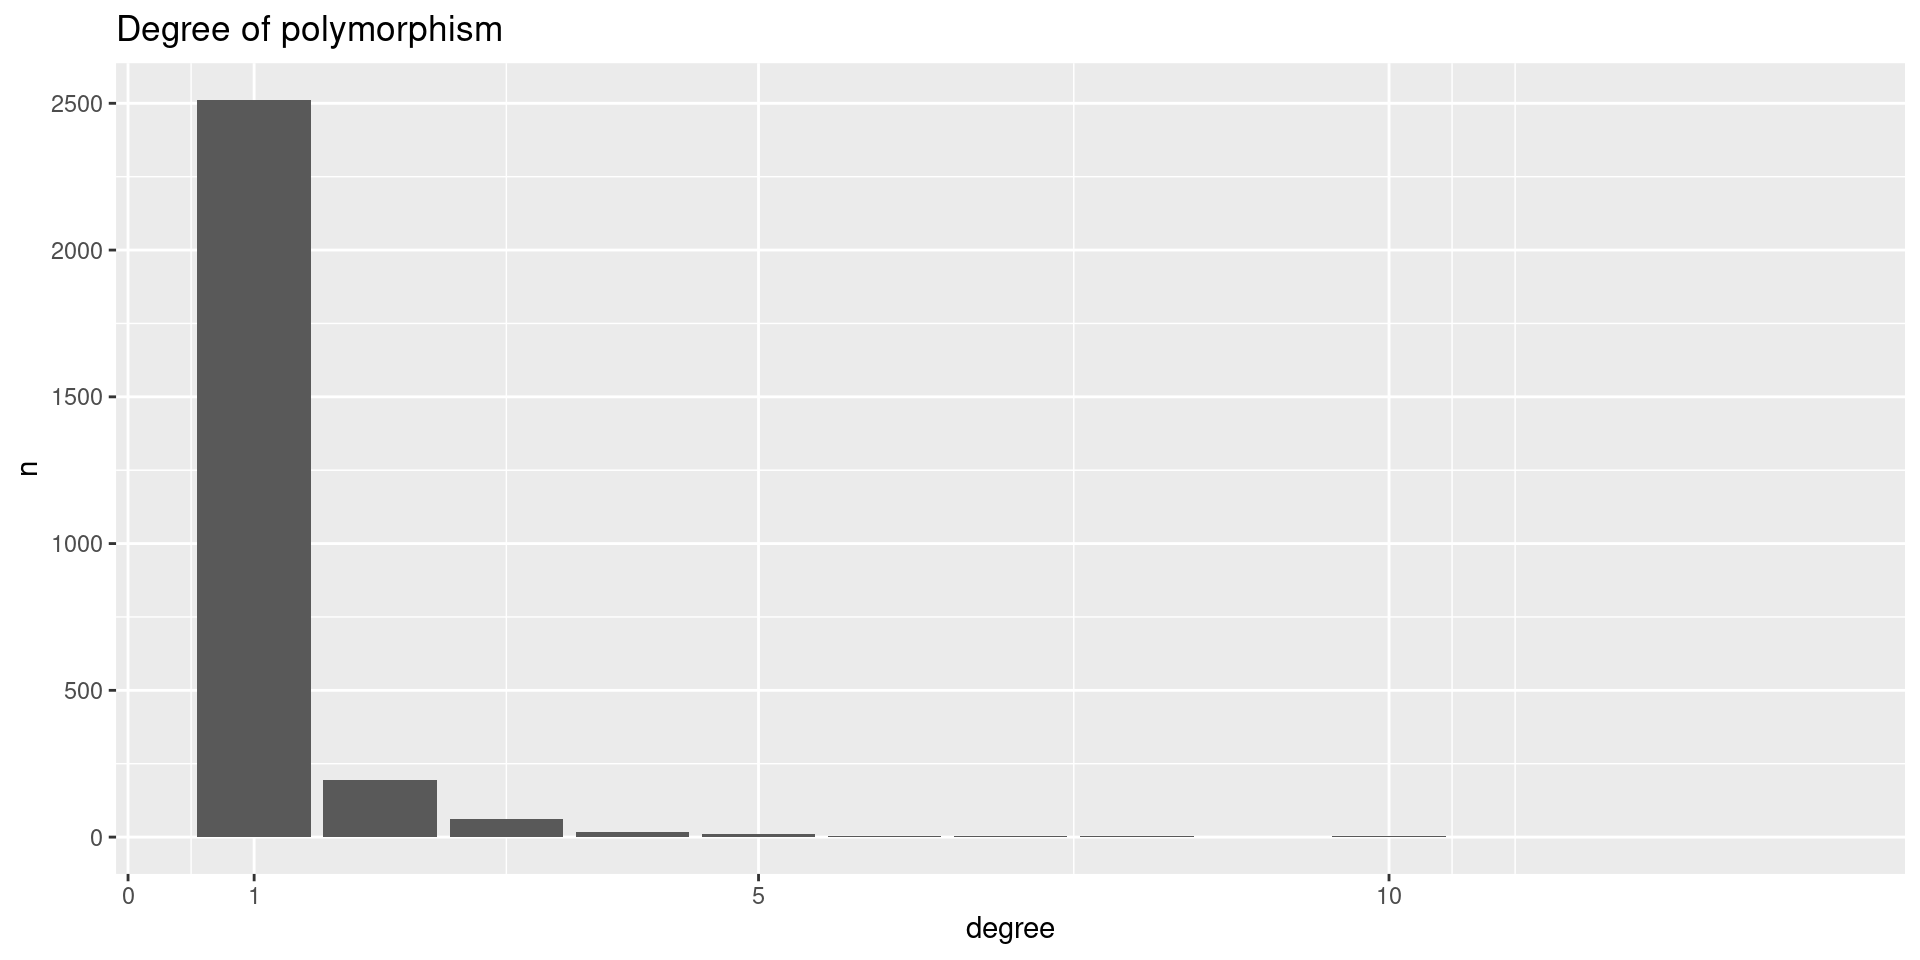
\includegraphics[width=\columnwidth]{polymorphism-1}
    \caption{Degree of polymorphism of \c{expr} per call sites.} \label{fig:polymorphism}
\end{figure}

\subsection{How dangerous is eval}

\subsection{How many evals can be replaced}

\section{Case studies}

\subsection{base}


\section{Conclusion}

\bibliographystyle{IEEEtran}
\bibliography{bib/bibliography,bib/jv}

\end{document}


Eval is evil, we would like to replace it.
Research Questions
How often is eval used? 
How often it is used in base / other packages?
blocking: cannot find out precisely what comes from base
What is the source of evals?
Provenance (source arguments to eval)
How many evals are in libraries / vignettes
What is eval used for?
??Eval in the tidyverse
TODO: Classification of evals in  packages (Pierre)
TODO: look at the first function to get
binary / unary / assignment / other function
does it have {
evals that do nothing (they get values)
...
TODO: In the case of base package (Filip)
access default values of formals
simply implementation
weird replacement of calls (write.csv -> write.table)
accessing variable from another environment (instead of get)
evaling user input
Change of caller pattern: 
m <- match.call()
 m$name <- NULL
 m[[1L]] <- as.name("library")
eval(m, .GlobalEnv)
     - 	TODO: How dangerous is eval? (Aviral)
Does eval generate new code (create new functions)?
environment writes (reads)
system environment variables
connections
random number generator - setting seed
Does eval do dynamic code loading?
Does eval argument reflect on the call stack?
Calls to C Code
TODO: Could the eval be made safer?
TODO: Could some of the eval calls be replaced?
